\documentclass[11pt,a4paper]{article}
% Journal-neutral draft. Swap the class and bibliography style for the
% target journal's template once one is chosen.
\usepackage[margin=2.4cm]{geometry}
\usepackage[T1]{fontenc}
\usepackage{lmodern}
\usepackage{microtype}
\usepackage{amsmath}
\usepackage{booktabs}
\usepackage{graphicx}
\usepackage{float}
\usepackage{xcolor}
\usepackage[numbers,sort&compress]{natbib}
\usepackage[hidelinks]{hyperref}
\graphicspath{{../../figures/}}

% Anything that waits on the registered grid or a later run.
\newcommand{\pending}[1]{\textcolor{red!70!black}{[\textbf{pending:} #1]}}
\newcommand{\todo}[1]{\textcolor{orange!80!black}{[\textbf{todo:} #1]}}
\newcommand{\cell}[1]{\texttt{#1}}

\title{Tumour-type conditioning, region-wise intensity augmentation and evaluation
protocol in 2D brain-tumour segmentation: a pre-registered study}
\author{Farzana Rahman Supti}
\date{Draft, 17 November 2026}

\begin{document}
\maketitle

\begin{abstract}
\pending{written last, after the H2--H4 results.}
\end{abstract}

\section{Introduction}

\todo{draft after results. The arc: (i) a pre-registered test of whether
conditioning the decoder on tumour type helps; (ii) the baseline credibility gate
failing, and what investigating it showed about evaluation protocol on this
benchmark; (iii) what a label-aware intensity augmentation actually teaches the
network. Contributions list goes here.}

\section{Related work}
\label{sec:related}

\subsection{The Cheng benchmark and how it is evaluated}

The Cheng dataset \citep{chengdata,cheng2015} contains 3064 T1-weighted
contrast-enhanced MRI slices from 233 patients, covering meningioma, glioma and
pituitary tumours. Every slice comes with a tumour mask, a tumour-type label and a
patient identifier. It was released for type classification \citep{cheng2015},
and it has since become a common testbed for 2D segmentation.

Studies on this dataset differ in a choice that strongly affects their results:
whether the data are split by patient or by slice. Several segmentation studies
describe their split only in slice or image counts. Gupta et al.\ divide the data
into ``train (2485 instances), validation (274 instances), and test (305
instances) sets'' \citep{gupta2023}. Rai et al.\ give image counts of
2482\,/\,337\,/\,245 \citep{rai2024}. Preetha et al.\ use a 90:10 split of the
3064 slices stratified by tumour type, and explain that they did not use
cross-validation \citep{preetha2025}. None of the three mentions grouping by
patient. Others state a patient-level split. Avazov et al.\ write that ``the
dataset was split on a patient ID basis, allocating 80\% for training and 20\% for
testing, to prevent data leakage'' \citep{avazov2024}. Yurdakul et al.\ use
stratified group five-fold cross-validation at patient level, and benchmark
fourteen architectures under one shared protocol \citep{yurdakul2026}. Under that
protocol, Dice ranges from 84.0 to 89.6, and a plain U-Net scores
$84.1\pm1.6$ \citep[Table~2]{yurdakul2026}. Their survey table classifies earlier
studies by split type. We follow each paper's own description wherever the two
disagree \citep[Table~1]{yurdakul2026}.

\subsection{Leakage, aggregation and variance in evaluation}

Splitting volumetric data at slice level puts near-identical neighbouring slices
of one patient on both sides of the evaluation boundary. Yagis et al.\ measured
this for 2D CNN classification of brain MRI. Slice-level cross-validation inflated
test accuracy by 29--55\% across four datasets. On randomly labelled data it
reached about 96\% accuracy, where a subject-level split gave chance
\citep{yagis2021}. More broadly, Kapoor and Narayanan count at least 294 papers
across 17 fields affected by leakage, and propose model info sheets to catch it
before publication \citep{kapoor2023}. Varoquaux and Cheplygina trace how data
choices, evaluation choices and publication incentives combine to bias
medical-imaging results \citep{varoquaux2022}.

Leakage is not the only source of disagreement between reported numbers. In an
analysis of 150 biomedical image-analysis challenges, Maier-Hein et al.\ show that
different aggregation methods produce different winners
\citep{maierhein2018}. Metrics Reloaded argues that metric
choice should follow from a structured description of the problem, not from
convention \citep{maierhein2024}. Variance from data sampling, initialisation and
hyperparameter choice is large enough that common comparison methods often detect
improvements that are not there \citep{bouthillier2021}. We add two measurements for segmentation on
this benchmark: how much the split unit and the aggregation convention move an
identical model, and how leakage changes the cross-validated variance itself.

\subsection{Conditioning segmentation on tumour type}

Feature-wise linear modulation (FiLM) conditions a network's intermediate features
on side information through a learned per-channel scale and shift
\citep{perez2018}. On the Cheng dataset, segmentation and type classification
have usually been treated as parallel tasks, for example as two heads on a shared
encoder \citep{rai2024}. We test a tighter coupling: the decoder is
FiLM-conditioned on the type posterior from the network's own classification
head. We also report an oracle variant conditioned on the true type, which bounds
what any type head could contribute. \todo{search for prior class-conditioned
decoders in medical segmentation before claiming novelty here.}

\subsection{Intensity augmentation with B\'ezier curves}

Models Genesis introduced smooth, monotonic cubic B\'ezier curves as a non-linear
intensity transform for medical images, as part of a self-supervised restoration
task \citep{zhou2021genesis}. Such transforms have since been used to simulate
appearance shift for single-source domain generalisation, mostly at the level of
the whole image \citep{zhou2022style}. Two methods make the transform
label-aware. SLAug applies constrained B\'ezier transforms separately to each
class region, cropped with the ground-truth mask. It combines the result with a
globally transformed image through a saliency-balancing fusion step
\citep{su2023slaug}. Yurdakul et al.\ remap tumour and background with
independent curves composed through the binary mask. They apply this with
probability 0.5, sample control points within a deviation bound of 0.5 around
the identity, and note that ``a narrow boundary band can be smoothed to avoid a
visible seam'' \citep{yurdakul2026}. They report that the region-wise variant
adds 1.5 Dice points over a global curve on the source domain, and more under
domain shift.

\subsection{Shortcut learning}

A network trained on any cue that separates the training labels will use that cue
whether or not it exists at test time \citep{geirhos2020}. Label-aware
augmentation creates one risk of this kind. If the transform is computed from the
ground-truth mask, the augmented image can carry the mask's outline as an
intensity edge, and test images never carry it. Section~\ref{sec:h3} measures how
strongly the region-wise transform used here does this, and what it costs.

\section{Methods}
\label{sec:methods}

\subsection{Pre-registration}
The analysis plan was committed to the project repository on 14 September 2026,
before any training run completed: hypotheses, outcomes, statistics, equivalence
margin, decision rules, stopping rule and a baseline credibility gate. Later
decisions were added only as dated deviations, and every such analysis is labelled
exploratory. \todo{repository URL and commit hash of the registration.}

\subsection{Data and splits}
Cheng dataset as above. Registered protocol: stratified group five-fold
cross-validation at patient ID (seed 42). Within each training portion, a
patient-disjoint validation set is carved out (70/10/20 overall). For the
protocol analysis only, a slice-level five-fold split of the same data is drawn
with the same seed. Under it, 224 of 233 patients span more than one fold.

\subsection{Models}
\textbf{U-Net} (31.0M parameters) as the unconditioned baseline.
\textbf{Conditioned U-Net}: the same encoder and decoder, plus a type-classification
head on the bottleneck. Each decoder block is FiLM-modulated by a
three-dimensional condition vector: the softmax type posterior (\emph{predicted}),
or the one-hot true type (\emph{oracle}). The loss is Dice+BCE with weight 0.5,
plus cross-entropy on the type head with weight 0.2.
FiLM computes $x\,(1+\gamma)+\beta$ at the output of every decoder stage. $\gamma$
and $\beta$ come from a linear projection of the condition vector, initialised to
zero, so the conditioned network starts as an exact copy of the unconditioned
one. Gradients flow through the posterior into the type head. The type head
average-pools the bottleneck, applies dropout of 0.1, and ends in a linear layer.

\subsection{Augmentation arms}
All arms share the same geometric augmentation (horizontal flip, rotation within
$\pm15^\circ$, scale within $\pm10\%$), drawn identically item by item across
arms. \emph{Standard} adds nothing. \emph{Global} remaps the whole image through
one random cubic B\'ezier curve. \emph{Region} remaps tumour and background, as
defined by the ground-truth mask, through two independent curves. Curves are
monotonic with probability 0.5, and otherwise order-reversing. As registered, the
B\'ezier arms apply on every training image, and control points are drawn from
the full unit square. Section~\ref{sec:h3} compares these settings with
\citet{yurdakul2026}.

\subsection{Training}
Input $192\times192$; micro-batch 8 with effective batch 16 by gradient
accumulation; AdamW (learning rate $10^{-4}$, weight decay $10^{-2}$); cosine
schedule; at most 150 epochs; early stopping on validation Dice with patience 20.
Initialisation is seeded per fold, so all arms within a fold start from the same
weights. One NVIDIA GTX 1650 (4\,GB).

\subsection{Outcomes and statistics}
Co-primary outcomes: slice-averaged and patient-averaged Dice on the held-out fold.
Secondary: IoU, HD95, ASSD and type accuracy. Each hypothesis is a paired
comparison over five fold-level differences. We report a paired $t$-test with
Cohen's $d_z$ and a 95\% CI, Holm-corrected across the four registered contrasts.
A claim of no difference requires TOST against a registered margin of
$\pm0.005$ Dice. Every configuration ran all five folds before its numbers were
examined.

\section{Results}

\subsection{Baseline and the credibility gate}
The U-Net baseline reached $0.7719\pm0.0164$ slice-averaged Dice
($0.7699\pm0.0286$ patient-averaged; 0.7846 pooled), 6.9 points below the 84.1
reported under the same split unit \citep{yurdakul2026}. The gate therefore failed.
An initial explanation through reporting conventions was withdrawn once the source
protocol had been checked (deviation of 17 November). The gap stays open, and
weight decay ($10^{-2}$ here, $10^{-4}$ in the source) is the main untested
difference. \pending{five-fold weight-decay $10^{-4}$ run, if done before submission.}

\subsection{Evaluation protocol}
\label{sec:protocol}

\begin{table}[H]
\centering\small
\begin{tabular}{@{}lcccc@{}}
\toprule
aggregation & patient-disjoint & slice-level & difference & sd ratio\\
\midrule
slice-averaged & $0.7719\pm0.0164$ & $0.8152\pm0.0035$ & $+0.0433$ & $4.8\times$\\
pooled & $0.7846\pm0.0165$ & $0.8358\pm0.0054$ & $+0.0511$ & $3.0\times$\\
patient-averaged & $0.7699\pm0.0286$ & $0.8152\pm0.0035$ & $+0.0453$ & $8.3\times$\\
\bottomrule
\end{tabular}
\caption{One U-Net, two split units (five folds each, unpaired).}
\label{tab:protocol}
\end{table}

A slice-level split adds 4.3--5.1 Dice points, and with pooled aggregation 6.4
points in total. Its larger effect is on the spread: the between-fold sd shrinks
3--8$\times$, because the folds no longer sample patients. The gain is
concentrated in glioma ($0.6627\to0.7344$; zero-Dice slices 133 $\to$ 88 of
1426). It does not grow with training length ($r=-0.21$, $n=5$). Fold 0 alone
understated the five-fold effect by three points.

\begin{figure}[H]
\centering
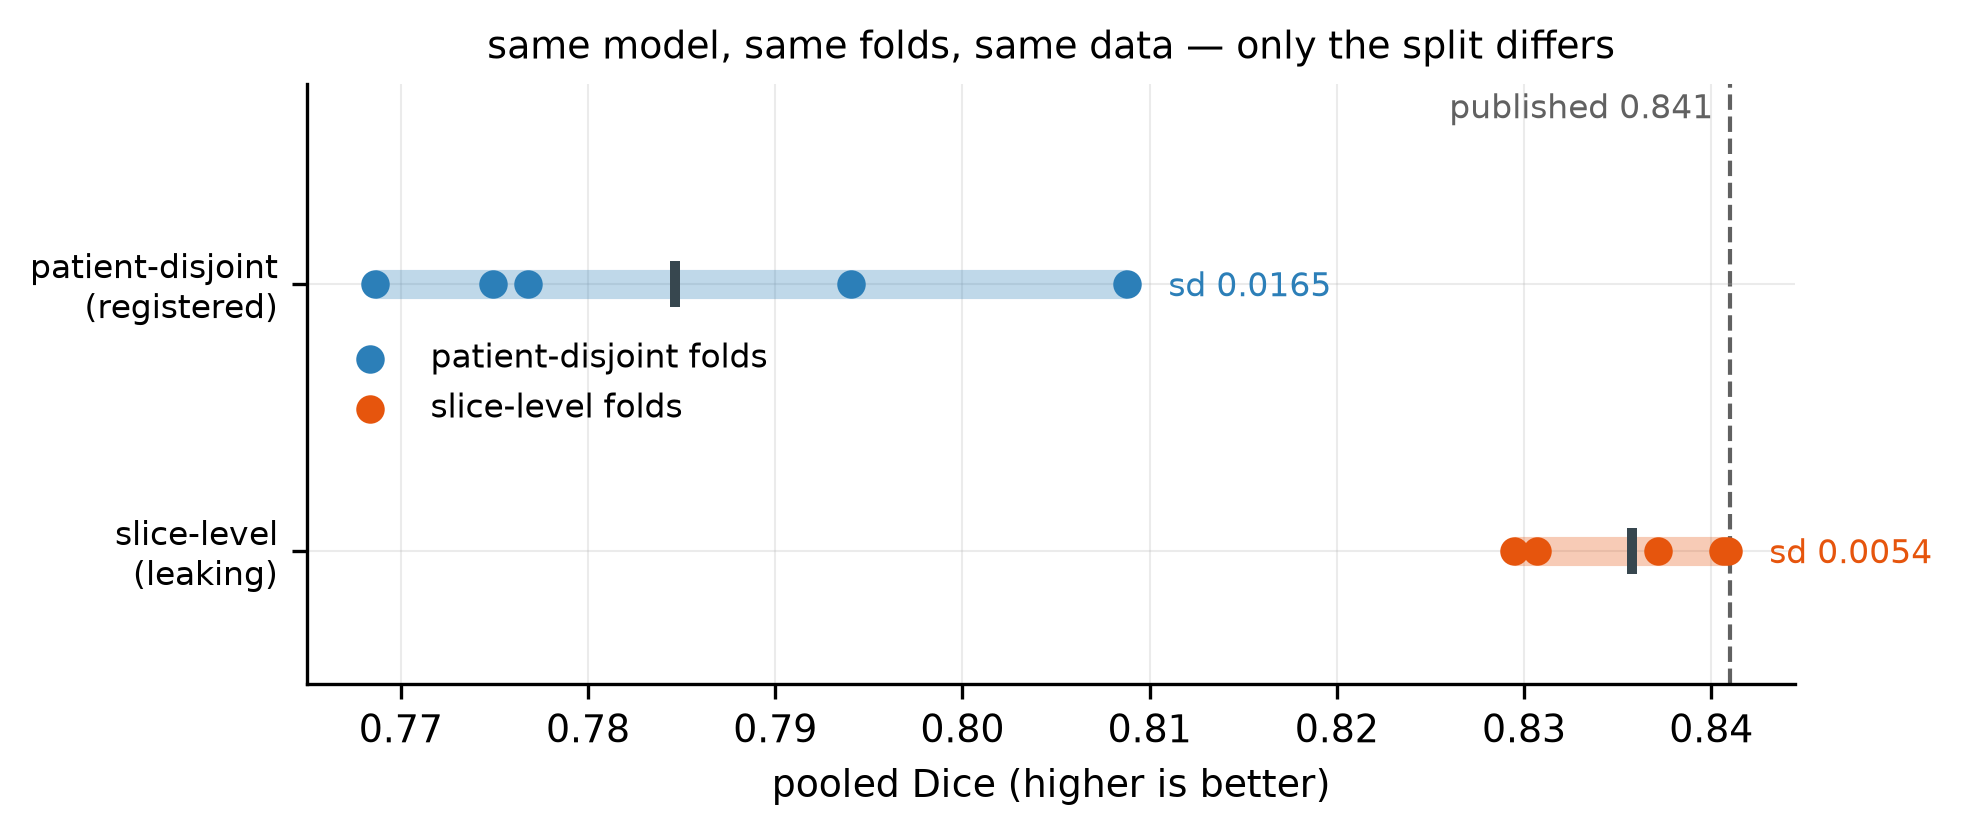
\includegraphics[width=0.49\linewidth]{protocol.png}\hfill
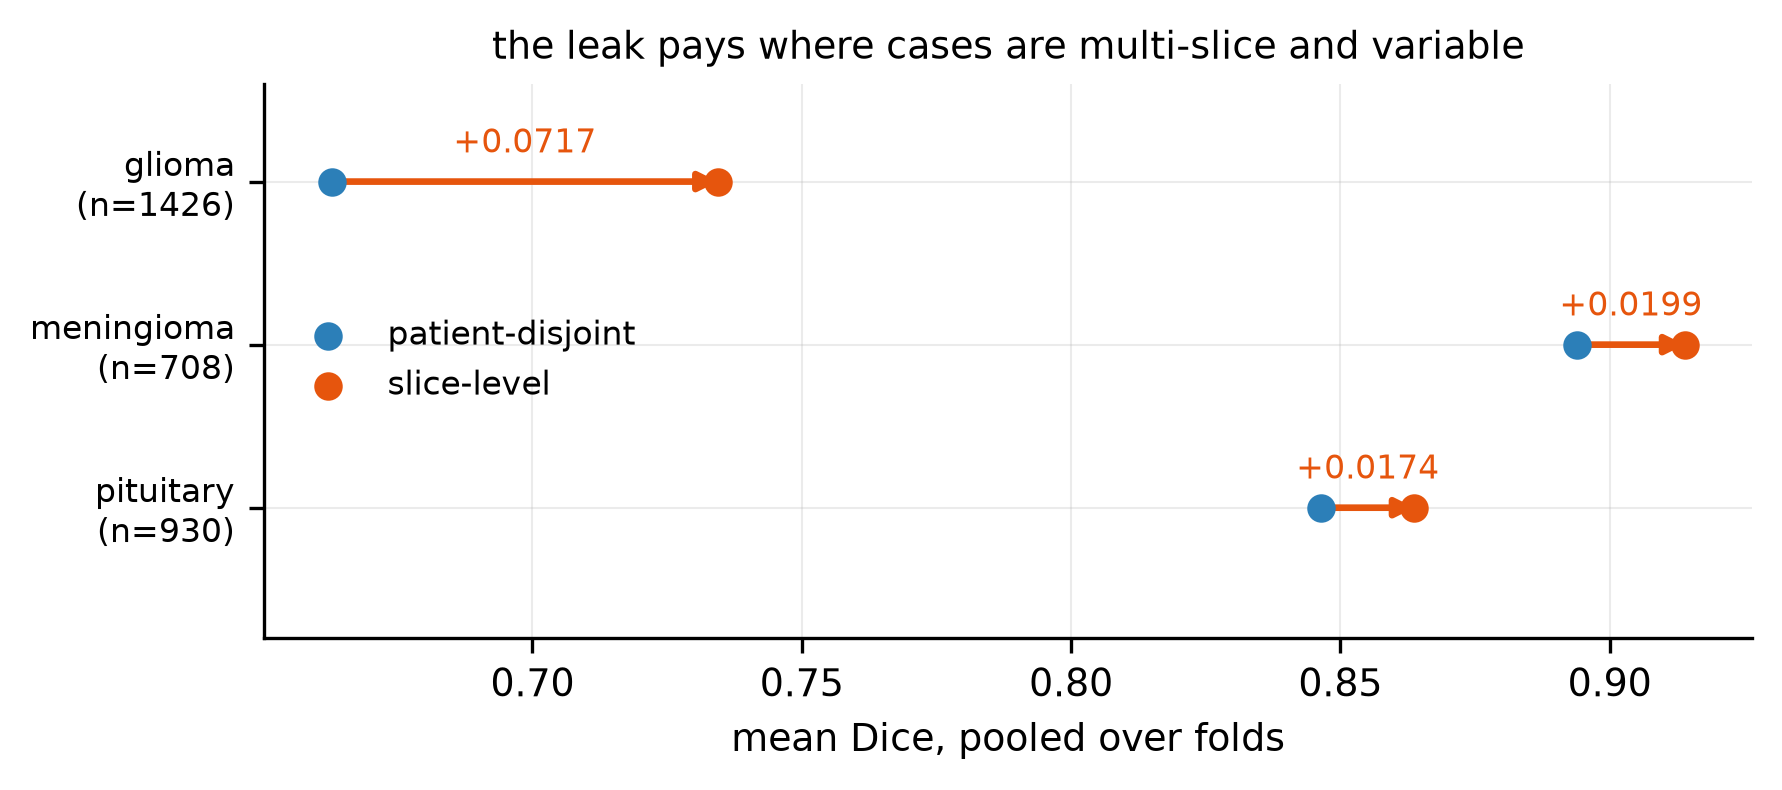
\includegraphics[width=0.49\linewidth]{protocol_by_type.png}
\caption{Left: per-fold pooled Dice under both split units. Right: by tumour type.}
\end{figure}

\subsection{H1: conditioning on the predicted type}

\begin{table}[H]
\centering\small
\begin{tabular}{@{}lccccc@{}}
\toprule
outcome & U-Net & conditioned & difference [95\% CI] & $p$ & TOST $p$\\
\midrule
slice-averaged Dice & 0.7719 & 0.7631 & $-0.0088\ [-0.025,+0.008]$ & 0.21 & 0.72\\
patient-averaged Dice & 0.7699 & 0.7551 & $-0.0147\ [-0.031,+0.001]$ & 0.063 & 0.92\\
\bottomrule
\end{tabular}
\caption{H1 over five paired folds. $p$ values before Holm correction ($m=4$).}
\end{table}

Under the registered decision rules, H1 is inconclusive. The point estimate is
negative on both co-primary outcomes and for every tumour type, even though the
type head reaches 93.8\% accuracy. \pending{Holm-adjusted $p$ across all four
contrasts.}

\subsection{H2: conditioning on the true type}
\pending{five folds; oracle $-$ predicted contrast. If the oracle also fails to
beat the plain U-Net, then type information does not help this decoder at all,
not merely imperfect type predictions.}

\subsection{H3 and H4: region-wise augmentation}
\label{sec:h3}

Before folds 1--4 ran, we measured how strongly each arm marks the label
boundary. Across 100 training slices, the median intensity step across the
tumour boundary, divided by the image standard deviation, was 0.39 for
\emph{standard}, 0.33 for \emph{global} and 1.55 for \emph{region}. The step
exceeded one standard deviation on 8\%, 3\% and 62\% of slices respectively. On
fold 0, the region arm reached a training loss of 0.014 but a test Dice of 0.5746,
against 0.7914 for the standard arm. Both the measurement and the prediction that
H3 and H4 would be negative were recorded before the remaining folds ran.
\pending{five-fold H3 and H4 contrasts.}

\section{Discussion}
\pending{after results. Points to cover: why type information does not help (or
does, if H2 says so); the protocol effect and what it means for cross-paper
comparison; label-aware augmentation as a source of shortcut learning, with the
settings that limit it; the open 84.1 gap.}

\section{Limitations}
One dataset, one architecture family, one seed per fold, and five folds, so
intervals are wide. The protocol comparison is unpaired. The registered region arm
perturbs more often and more strongly than \citet{yurdakul2026}, so a negative H3
describes this implementation, not theirs. \pending{corrected-arm result, if run.}

\section{Conclusion}
\pending{after results.}

\section*{Data and code availability}
\todo{repository URL; the dataset is public \citep{chengdata}.}

\bibliographystyle{unsrtnat}
\bibliography{refs}

\end{document}
